\chapter{Métodos}

Para responder a primeira questão estudou-se o comportamento do parâmetro p na equação publicada pela ENTSO-E para a Banda de Regulação Secundária a Subir \cite{CMVM2018}:
\begin{equation}
\label{eq:eq_entso-e}
    BRSsubir = p \times \sqrt{a \times Lmax + b^2} - b 
\end{equation}
TODO: explicação das variaveis

Aplicando os dados XXXX (dados históricos do mercado MIBEL), 

Usandos os dados XXXXX para o calculo directo do parâmetro p e comparando com o mesmo parâmetro apresentado na tese de Célia Carneiro \cite{Carneiro2016}, temos a seguinte distribuição de valores:

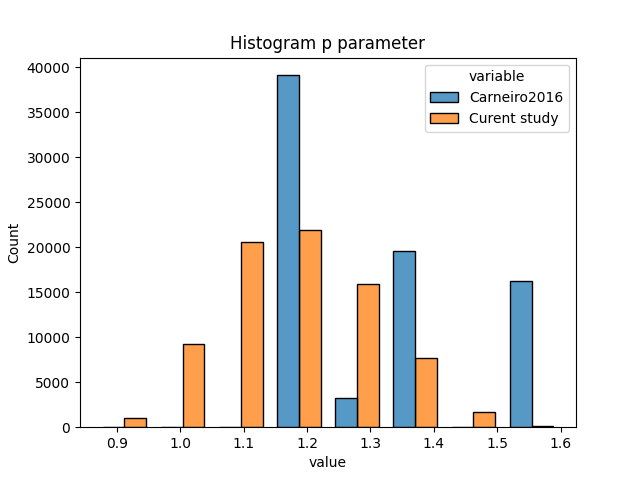
\includegraphics{Imagens/Histogram p parameter.png}
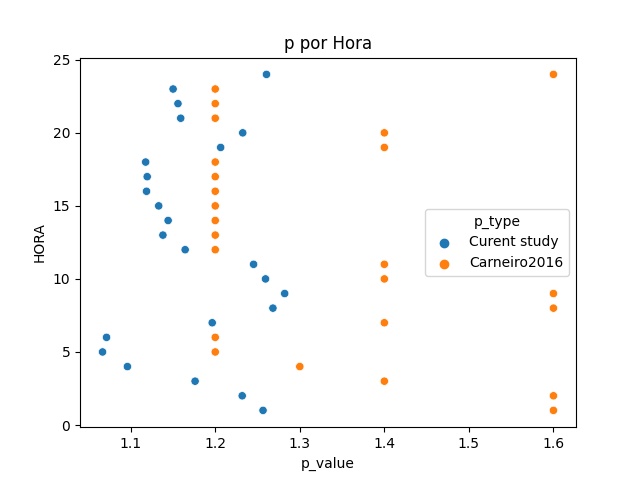
\includegraphics{Imagens/p por Hora.png}

Verifica-se que não têm qualquer relação entre si.

Para a normalização deste parâmetro à Hora, estudou-se o erro entre a Banda a Subir calculada através das normalizações e a Banda a Subir disponível nos dados. 

\begin{table}[H]
\centering
\caption{Isto é um exemplo de uma tabela. Se fôr igual(copiada) a outro autor deve ser pedido autorização para reproduzir.}
\begin{tabular}{p{5cm}p{3.5cm}p{2cm}p{2cm}}
\toprule %thicker line
\textbf{Normalização/Erro} & \textbf{MAE} & \textbf{RMSE} & \textbf{Mediana AE} \\ \hline
\multirow{1}{*}{media}   & 23.03 & 29.15 & 19.04            \\ \hline
\multirow{1}{*}{mediana}   & 22.95 & 29.14 & 18.93            \\ \hline
\multirow{1}{*}{media ponderada}   & 23.39 & 29.57 & 19.28            \\ \hline
\end{tabular}
\end{table}

A normalização que traz erros mais baixos à Banda é a mediana.
Comparando com os p \cite{Carneiro2016}: 

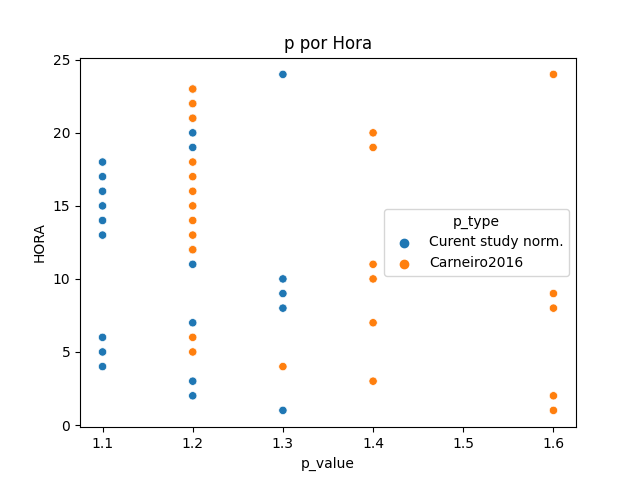
\includegraphics{Imagens/p por Hora norm.png}

Podemos verificar que os valores não coincidem.
Comparando as bandas calculadas:

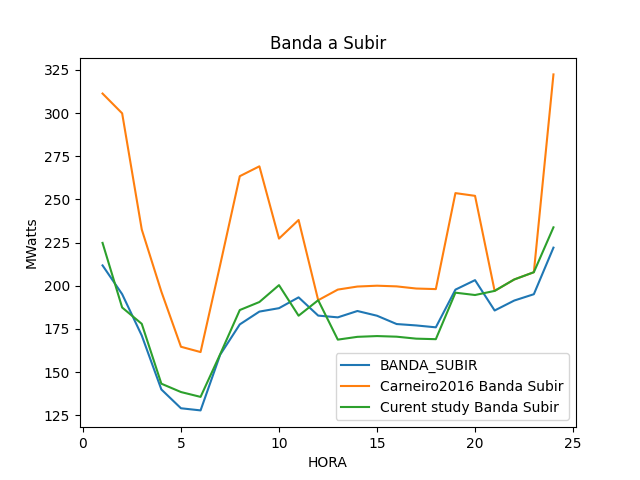
\includegraphics{Imagens/Banda a Subir.png}

Retiramos as médias dos erros percentuais e podemos observar em:

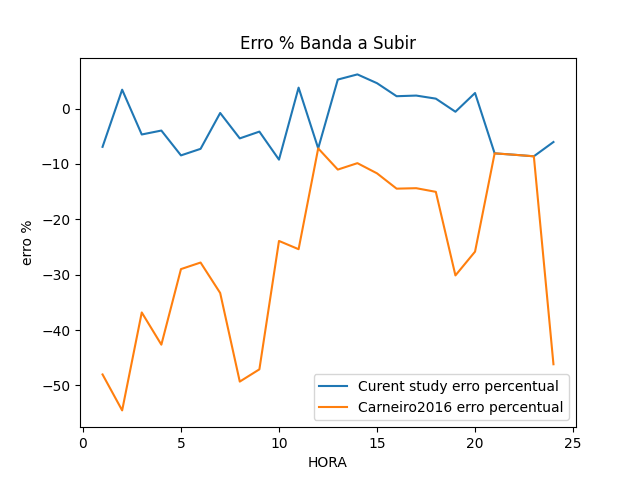
\includegraphics{Imagens/Erro per Banda a Subir.png}

Que conclui que o p calculado agora tem uma prestação bastante mais perto da realidade. 
Onde cerca de 25\% dos casos cai dentro da margem de erro de 5\% na Banda. E na outra tese apenas 10\% cai dentro dessa margem de erro.



Aqui descrever qual o método seguido para responder às perguntas de investigação, o método pode incluir o recurso a uma metodologia reconhecida internacionalmente e já publicada por exemplo numa norma ISO\cite{fet_skaar_2006}.
As figuras e tabelas colocadas devem ser sempre referidas no meio do texto tal como todas as referências que aparecem listadas no fim do documento. 



\section{Modelos estatiscos  \label{se:dados_estudo}}

\subsection{subsection ARIMA (depth 2)}

\subsection{subsubsection Gerador de dados (depth 2)}
distribuiçao

clustering




\section{Forecat  \label{se:dados_estudo}}

\subsection{subsection Construtor de modelos (depth 2)}

\subsection{subsubsection Gerador de dados (depth 2)}
distribuiçao

clustering


\section{Forecat  \label{se:dados_estudo}}

\subsection{subsection Construtor de modelos (depth 2)}

\subsection{subsubsection Gerador de dados (depth 2)}
distribuiçao

clustering


